%\subsection{A guided example...}
\subsection{Reading data...}
\begin{frame}
\frametitle{\href{https://wci.llnl.gov/simulation/computer-codes/visit/}{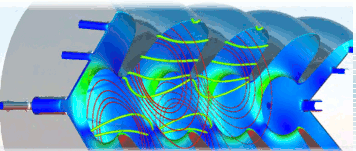
\includegraphics[height=.85cm]{figs/visit-logos/VisIt-02}} \hspace{-.85cm}{\bf \textcolor{lightgray}{VisIt}}: Import Data}

\begin{columns}
\begin{column}{6.25cm}
        \textcolor{DarkRed}{*} Importing datasets

        \textcolor{DarkBlue}{$\blacktriangleright$}
        \framebox{File} $\rightarrow$ \framebox{\bf Open file...}

        \hspace{2mm} $\mapsto$ choose data file {\small (eg. ``\textcolor{gray}{noise.silo}'')}

        \pause
        \vspace{2mm}
        \begin{beamerboxesrounded}[upper=block head,lower=block body,shadow=true]{\ding{231} Become available}
                \hspace{2mm}
                \ding{232} \textcolor{DarkBlue}{Active source}: ``\textcolor{gray}{noise.silo}''

                \hspace{2mm}
                \ding{232} \textcolor{DarkBlue}{Add button}
        \end{beamerboxesrounded}

        \pause
        \vspace{2mm}
        \textcolor{DarkBlue}{$\blacktriangleright$}
        \framebox{File} $\rightarrow$ \framebox{\bf File information...}
\end{column}
\begin{column}{5.5cm}
        \textcolor{DarkRed}{*} Restoring a previous session

        \vspace{2.5mm}
        \textcolor{DarkBlue}{$\blacktriangleright$}
        \framebox{File} $\rightarrow$ \framebox{\bf Restore session...}
        \\
        loads the previous state of the given session (\textbf{that needs to be specifically saved})

        \vspace{3.5mm}
        \textcolor{DarkBlue}{$\blacktriangleright$}
        \framebox{File} $\rightarrow$ \framebox{\bf Restore session w/sources...}
        \\
        extremely useful for re-identifiying datasets that could have been moved or renamed
        %\centering
        %\includegraphics[width=.85\columnwidth]{figs/}
\end{column}
\end{columns}
\pause
\vspace{2mm}
\begin{beamerboxesrounded}[upper=block head,lower=block body,shadow=true]{}
Be aware, that VisIt, by default won't save your work (session) nor ask you when you try to exit the program!
\end{beamerboxesrounded}
\end{frame}




\subsection{Contours: Iso-Surfaces \& Iso-Curves}
\begin{frame}
\frametitle{\href{https://wci.llnl.gov/simulation/computer-codes/visit/}{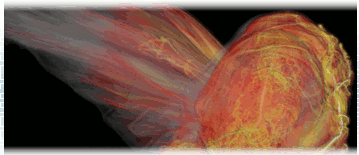
\includegraphics[height=.85cm]{figs/visit-logos/VisIt-03}} \hspace{-.85cm}{\bf \textcolor{lightgray}{VisIt}}: Contours}

\begin{columns}
\begin{column}{5cm}
        \textcolor{DarkBlue}{$\blacktriangleright$}
        \framebox{Add$_\blacktriangledown$} $\rightarrow$ \framebox{Contours}

        \hspace{5.5mm}
        $\leadsto$ \framebox{\textcolor{DarkGreen}{\it hardyglobal}}

        \hspace{5.5mm}
        $\rightarrow$ \framebox{\textcolor{DarkBlue}{Draw}}

        \centering
        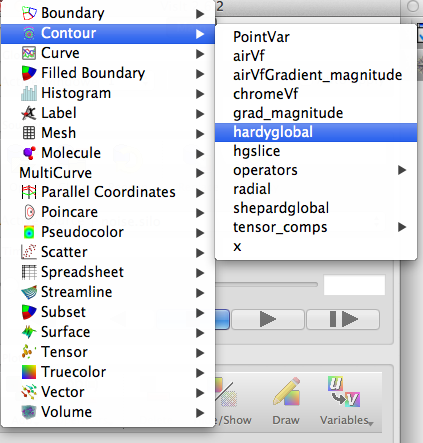
\includegraphics[width=\columnwidth]{figs/visit-pract/VisIt_contour}
\end{column}
\begin{column}{6.5cm}
        \centering
        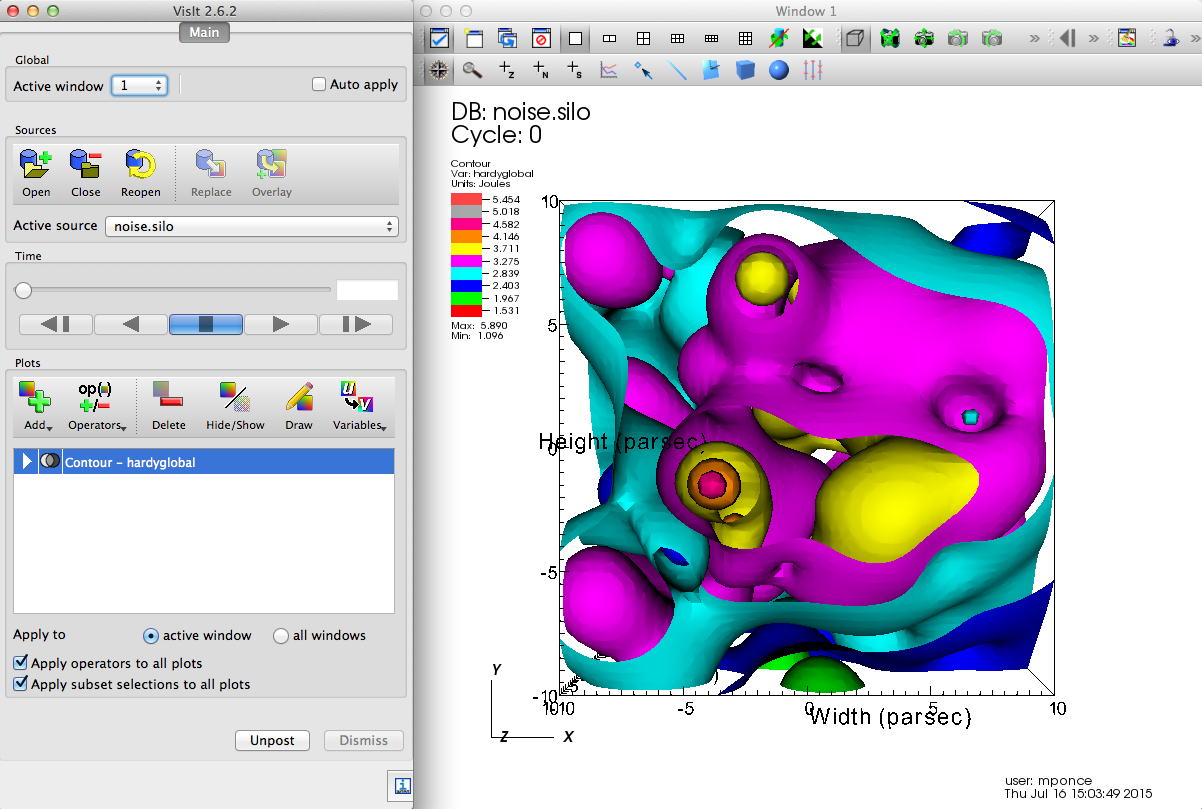
\includegraphics[width=\columnwidth]{figs/visit-pract/VisIt_contour1a}
\end{column}
\end{columns}
\end{frame}


\begin{frame}
\frametitle{\href{https://wci.llnl.gov/simulation/computer-codes/visit/}{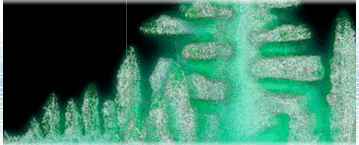
\includegraphics[height=.85cm]{figs/visit-logos/VisIt-04}} \hspace{-.85cm}{\bf \textcolor{lightgray}{VisIt}}: Contours}

\begin{columns}
\begin{column}{6cm}
        \textcolor{DarkBlue}{\ding{224}}
        double-click on \textcolor{DarkGreen}{Contour-hardyglobal}

        \pause
        \textcolor{DarkBlue}{\ding{224}}
        under \textcolor{DarkBlue}{Select by}, choose \framebox{\textcolor{DarkGreen}{N levels}} = \textcolor{blue}{5} \Enter

        \pause
        \textcolor{DarkBlue}{\ding{224}}
        Change \textcolor{DarkBlue}{opacity levels}, eg: 100\%, 60\%, 60\%, 48\%, 24\%

        \centering
        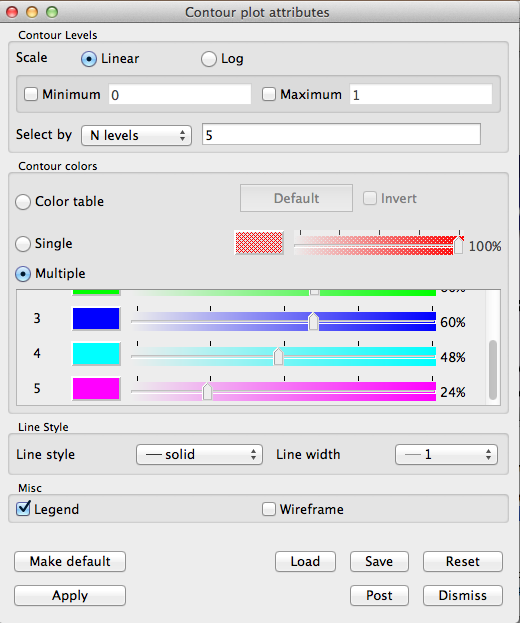
\includegraphics[width=.65\columnwidth]{figs/visit-pract/VisIt_contour-props}
\end{column}
\begin{column}{5.5cm}
        %\pause
        \textcolor{DarkBlue}{\ding{224}}
        \framebox{Apply}
        \&
        \framebox{Dismiss}

        \vspace{3mm}
        %\centering
        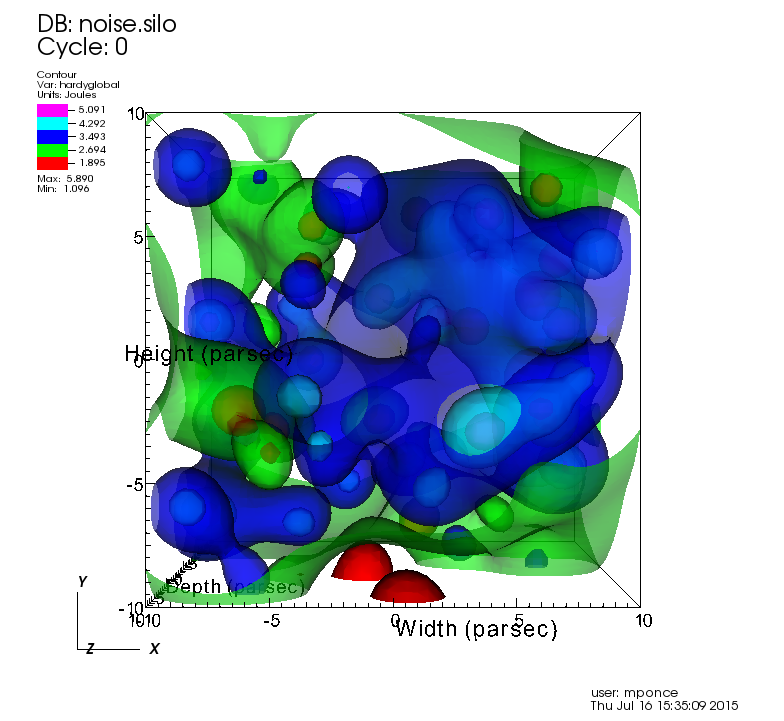
\includegraphics[width=\columnwidth]{figs/visit-pract/VisIt_contour1b}

        \pause
        \vspace{3mm}
        %\left
        \textcolor{DarkBlue}{\ding{224}}
        \framebox{Hide/Show}
        or
        \framebox{Delete}
\end{column}
\end{columns}
\end{frame}

\begin{frame}
\frametitle{\href{https://wci.llnl.gov/simulation/computer-codes/visit/}{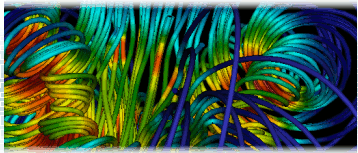
\includegraphics[height=.85cm]{figs/visit-logos/VisIt-01}} \hspace{-.85cm}{\bf \textcolor{lightgray}{VisIt}}: PseudoColor \& IsoSurfaces}
\vspace{-1.85mm}
\begin{columns}
\begin{column}{6cm}
        \textcolor{DarkBlue}{\ding{224}}
        \framebox{Add$_\blacktriangledown$} $\rightarrow$ \framebox{\textcolor{DarkRed}{\bf Pseudocolor}}

        \hspace{5.5mm}
        $\leadsto$ \framebox{\textcolor{DarkGreen}{\it hardyglobal}}

        \hspace{5.5mm}
        $\rightarrow$ \framebox{\textcolor{DarkBlue}{Draw}}

        \centering
        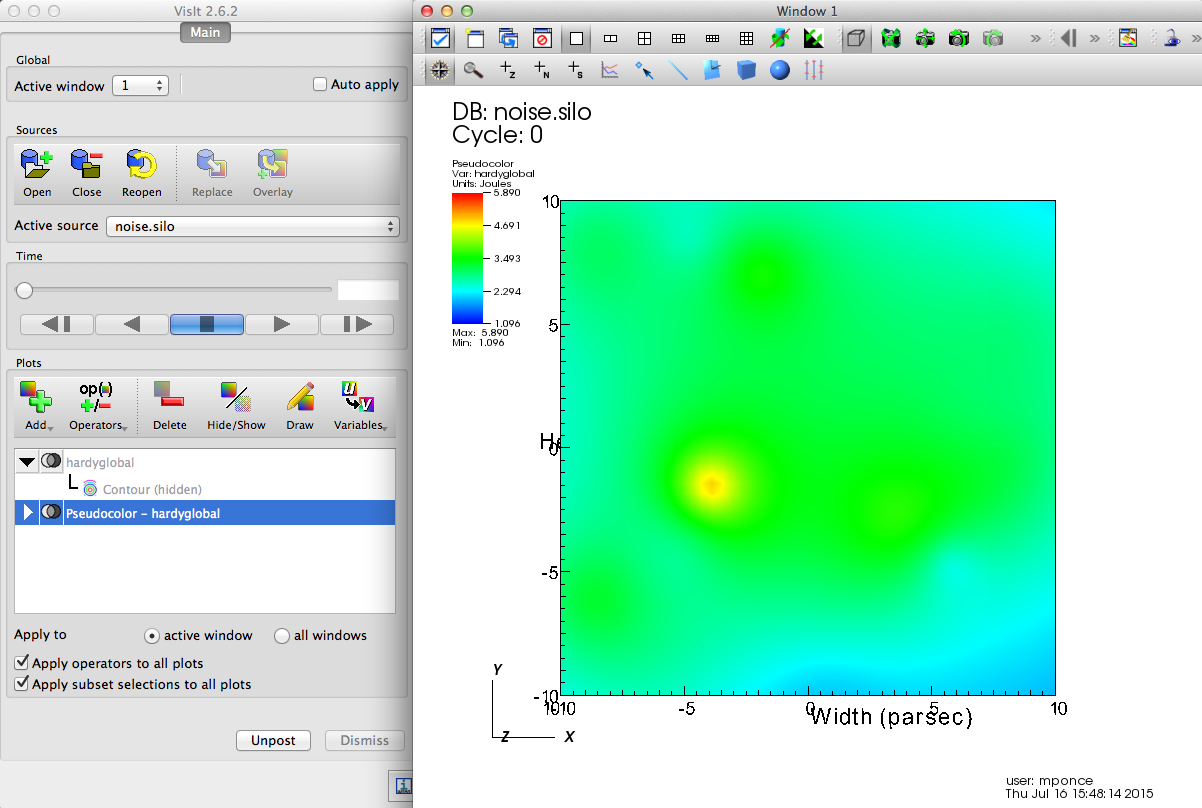
\includegraphics[width=\columnwidth]{figs/visit-pract/VisIt_pseudocolor}
\end{column}
\begin{column}{6cm}
        \pause
        \textcolor{DarkBlue}{\ding{224}}
        \framebox{Operators$_\blacktriangledown$}
                $\rightarrow$ \framebox{\bf Slicing}

        \hspace{5.5mm}
        $\rightarrow$ \framebox{\textcolor{DarkRed}{\bf Isosurface}}

        \hspace{5.5mm}
        $\rightarrow$ \framebox{\textcolor{DarkBlue}{Draw}}

        \centering
        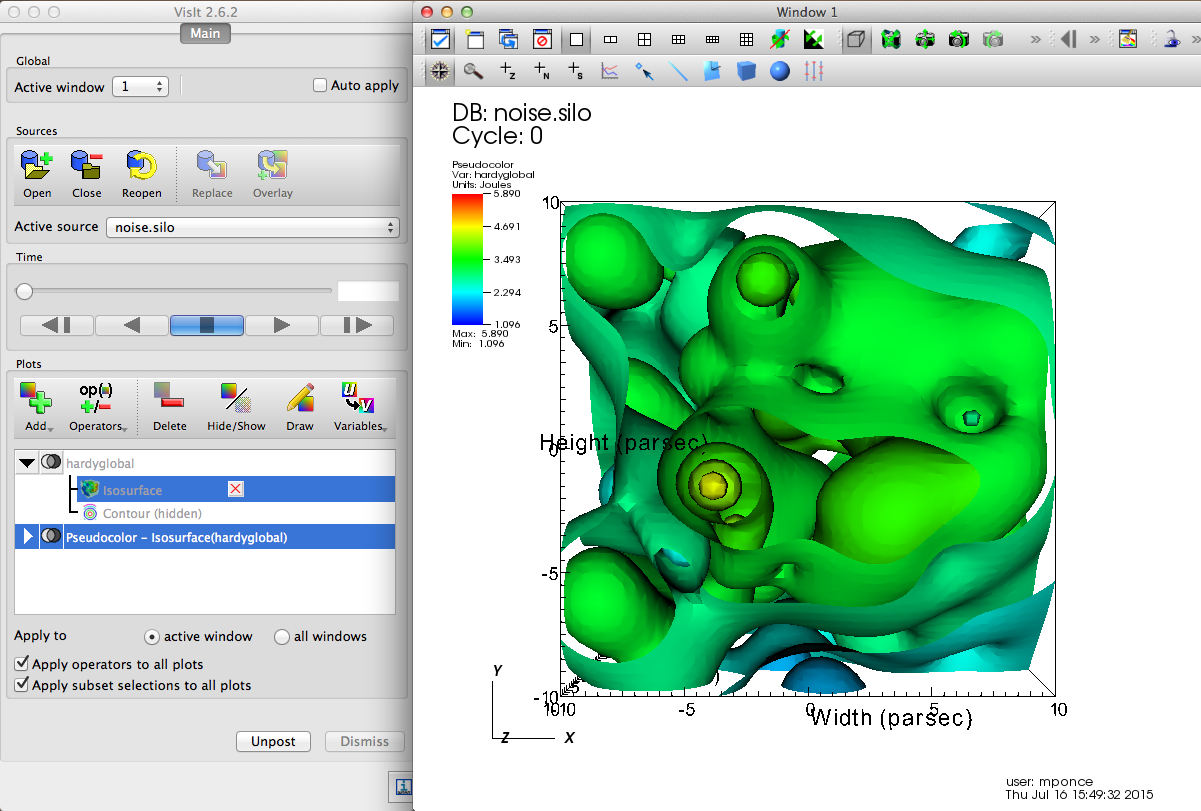
\includegraphics[width=\columnwidth]{figs/visit-pract/VisIt_pseudocolor-isosurf}
\end{column}
\end{columns}

\pause
\vspace{2mm}
\textcolor{DarkBlue}{\ding{224}}
        click $\blacktriangleright$ to expand, double click on [\textcolor{DarkBlue}{Isosurface}]

\hspace{4mm}
\textcolor{DarkBlue}{\ding{223}}
under \textcolor{DarkBlue}{Select by}, choose \framebox{\textcolor{DarkGreen}{Percent (s)}} = \textcolor{blue}{50} \Enter \& \framebox{Dismiss}


\pause
\vspace{2mm}
\textcolor{DarkBlue}{\ding{224}}
        change the \textcolor{DarkRed}{opacity} of [\textcolor{DarkBlue}{Pseudocolor}]
\end{frame}


\begin{frame}
\frametitle{\href{https://wci.llnl.gov/simulation/computer-codes/visit/}{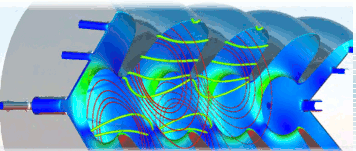
\includegraphics[height=.85cm]{figs/visit-logos/VisIt-02}} \hspace{-.85cm}{\bf \textcolor{lightgray}{VisIt}}: PseudoColor \& IsoSurfaces}
\vspace{-1.5mm}
\begin{columns}%[T]
\begin{column}{9cm}
        \centering
        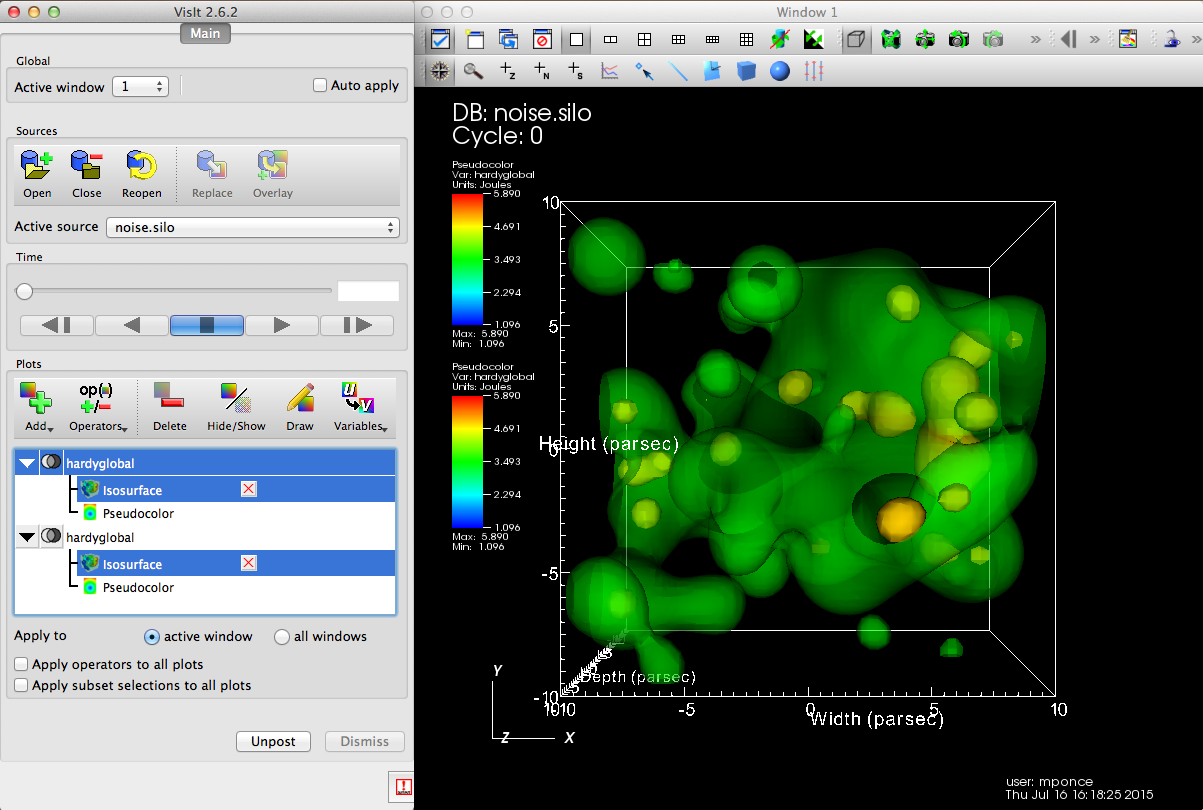
\includegraphics[width=\columnwidth]{figs/visit-pract/VisIt_pseudocolor-isosurf_2}
\end{column}
\begin{column}{3cm}
        \pause
        \textcolor{DarkBlue}{\ding{224}}
        unselect the [\textcolor{DarkBlue}{Apply ...}] check-boxes

        \vspace{2mm}
        \textcolor{DarkBlue}{\ding{224}} add 1 more
                \textcolor{DarkRed}{Pseudocolor}
                +\textcolor{DarkRed}{\bf Isosurface},
        \\
        %\hspace{1.5mm}
        w/\textcolor{DarkBlue}{Percent(s)=80}
        \& adjust its
        \textcolor{DarkBlue}{opacity}
\end{column}
\end{columns}

\pause
\vspace{2mm}
\textcolor{DarkBlue}{\ding{224}}
        \textcolor{blue}{clipping} \ding{223} select/check the [\textcolor{DarkBlue}{Apply...}] boxes

%\vspace{1mm}
\textcolor{DarkBlue}{\ding{224}}
        \framebox{Operators$_\blacktriangledown$}
                $\rightarrow$ \framebox{\bf Selection}
        %\hspace{5.5mm}
        $\rightarrow$ \framebox{\textcolor{DarkRed}{\bf Clip}}

        \hspace{5mm}
        \ding{223} choose \textcolor{DarkBlue}{combinations of $\ne$ planes} to modify the $\ll$clip$\gg$
\end{frame}















\begin{frame}
\frametitle{\href{https://wci.llnl.gov/simulation/computer-codes/visit/}{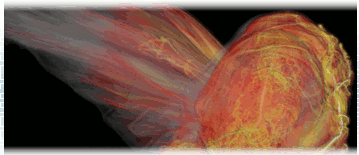
\includegraphics[height=.85cm]{figs/visit-logos/VisIt-03}} \hspace{-.85cm}{\bf \textcolor{lightgray}{VisIt}}: General Remarks}

\begin{beamerboxesrounded}[upper=block head,lower=block body,shadow=true]{}
        \textcolor{DarkBlue}{\ding{231}} operators/plots can be removed
                \framebox{\textcolor{DarkBlue}{\bf Delete}}
                --or--
                hidden \framebox{\textcolor{DarkBlue}{\bf Hide/Show}}

        \textcolor{DarkBlue}{\ding{231}} save your work {\bf frequently}:
                \framebox{File} $\rightarrow$ \framebox{\textcolor{DarkBlue}{\bf Save session...}}
\end{beamerboxesrounded}

\pause
\vspace{3mm}
\begin{beamerboxesrounded}[upper=block head,lower=block body,shadow=true]{Hands-on...}%Assignment ii}
        \textcolor{DarkRed}{\ding{231}} try loading some of the datasets we used with ParaView [{\small \textcolor{gray}{\tt headsq.vtk}, \textcolor{gray}{\tt testRectilinearGrid.vtk}, \textcolor{gray}{\tt disk\_out\_ref.ex2}, ...}] --or-- your own data!!!

        \textcolor{DarkRed}{\ding{231}} and compare how easy/possible or not, is to obtain similar results, let's say, to ParaView for instance...

        \textcolor{DarkRed}{\ding{231}} also which one, results more intuitive, elegant, useful for you and your research
\end{beamerboxesrounded}
\end{frame}

